
To find out whether sharing the clause database was beneficial to the
same-chip portfolio-approach solver, we ran AzuDICI in three different
versions (sharing all the clauses, sharing none of the clauses and
sharing only binaru clauses) on eight representative problems
(XXXNAMESXXX) using one to six threads. Each run was repeated five
times to clean up potential system noise. XXXKeiraXXX

\subsection{Same search experiments}
\label{sec:samesearch}

For this experiment, AzuDICI was modified to carry out the {\em same}
search in each thread (i.e., there is no lemma sharing among
threads). For each AzuDICI version, we measured the time needed to
solve each benchmark, and the percentage of LLC misses. The results
for this are shown in Table \ref{tbl:table} below.

Notice that the datasets we chose for this experiment were influenced
by the early state of the implementation of AzuDICI. Our solver is not
optimized, and has been implemented for the purposes of
experimentation for this paper. Thus, the datasets are generally
``easier'' for AzuDICI to solve.

  \begin{table}[h]
   \scriptsize
    \centering
    \begin{tabular}[h]{rcccccc} \hline
      Dataset  &  T1 &  T2 & T3  & T4  &  T5 &   T6\\ \hline
      \multirow{3}{*}{c10b} &         82.6(0.1)  &   95.8(0.1)  &   109.9(0.0) &   120.4(0.0)  &  130.5(0.0)  &  137.3(0.1)  \\
         & 84.4(0.2)   &  96.1(0.5)  &   108.1(0.4)   &   118.1(0.5)  &    126.6(0.3)   &   133.3(0.1)    \\
     &89.2(0.2)   &   99.1(0.5)   &    110.8(0.4)     &   118.9(0.6) &    128.3(0.7)  &  136.4(0.2)  \\ \hline
      \multirow{3}{*}{c6bid\_i}   &     255.0(0.0)  &  299.6(0.1)  &  337.8(0.0)  &  365.9(0.1)  &  391.7(0.1)  &  409.7(0.0)  \\
         & 262.4(0.0) &   301.9(0.4)  &  338.1(0.3)    &  365.8(0.3)   &   389.0(0.5)   &   407.4(0.1)    \\
    & 275.7(0.1)  &   308.3(0.7)   &    338.1(0.1)    &    365.4(0.5)   &  389.1(0.1)  &  421.6(0.1)  \\ \hline
      \multirow{3}{*}{c6nidw\_i}  &   298.9(0.0)  &  352.4(0.1)  &  396.9(0.0)  &  429.0(0.1)  &  461.5(0.2)  &  479.9(0.1)  \\
      &   307.8(0.1)  &  357.5(0.4)  &  398.7(0.2)  &    428.6(0.5)  &    456.2(0.1)   &   476.9(0.1)    \\
    & 324.5(0.0)  &   363.9(0.6)    &   397.2(0.0)   &     427.6(0.1)  &   456.5(0.1)  &  492.0(0.3)  \\ \hline
      \multirow{3}{*}{c7idw}    &   70.9(0.0)   &  84.5(0.1)   &  94.1(0.0)   &  100.6(0.0)  &  106.7(0.0)   & 110.7(0.1)  \\
     &    75.1(0.0)  &   86.7(0.6) &    95.4(0.7) &      102.5(0.2)   &   105.6(0.6)    &  111.5(0.6)    \\
     & 78.2(0.1)  &    89.7(0.7)   &     96.7(0.1)     &   102.6(0.1)   &  108.2(0.1)  &  114.9(0.5)  \\ \hline
      \multirow{3}{*}{05-113}   &     60.2(0.0)  &   68.5(0.1)   &  77.3(0.2)  &   84.7(0.1)  &   92.0(0.1)   &  96.8(0.1)   \\
      &   61.0(0.1)  &   68.4(0.2)  &   75.8(0.2)    &   82.4(0.2)   &    88.2(0.1)    &   93.2(0.1)     \\
    & 64.5(0.2)  &    71.7(0.2)   &     78.6(0.7)    &     83.1(0.3)   &   89.1(0.3)   &  94.6(0.3)  \\ \hline
      \multirow{3}{*}{5-15-u}    &    1146.8(0.1)  & 1440.9(0.1)  & 1709.0(0.0)  & 1914.7(0.2)  & 2075.7(0.0)  & 2188.7(0.1) \\
     &    1175.2(0.1) &  1457.9(0.1) &  1704.3(0.0)   &  1882.3(0.0)   &  2033.7(0.1)    & 2124.4(0.0)   \\
   & 1142.8(0.8)  &  1314.8(0.2)   &   1583.4(1.8)   &    1719.7(0.9)  &  1872.0(0.4)  & 1994.1(0.3)  \\ \hline
      \multirow{3}{*}{1r3-k30}   &    1569.5(0.1)  & 1733.0(0.1)  & 1912.2(0.0) &  2027.9(0.0)  & 2158.0(0.1)  & 2223.4(0.2) \\
    &     1581.1(0.0)  & 1737.1(0.1)  & 1912.9(0.0)  &   2021.0(0.1)  &   2138.9(0.1)   &  2193.3(0.0)   \\
   & 1624.4(0.2)   & 1769.8(0.2)   &   1889.8(0.3)   &    2003.4(0.5)   & 2104.6(0.2) &  2182.8(0.2)  \\ \hline
      \multirow{3}{*}{16-22}   &    966.9(0.0)  &  1050.1(0.2)  & 1134.0(0.0)  & 1189.0(0.0) &  1254.1(0.0) &  1281.7(0.0) \\
    &     973.0(0.0)   & 1046.9(0.3)  & 1134.1(0.1)  &   1185.0(0.1)   &  1245.3(0.2)   &  1267.9(0.1)   \\
   & 1004.2(0.0)  &  1069.1(0.6)   &   1156.5(0.2)    &   1204.1(0.2) &   1264.5(0.2)  & 1293.7(0.2)  \\ \hline
    \end{tabular}
    \normalsize
    \caption{Runtime (seconds) for AzuDICI and number of threads (T). 
      The first row of each dataset is the Shared-None version, the second row is the Shared-Binaries version and the third row is the Shared-All version. Numbers in parenthesis are standard deviations in \%.}
    \label{tab:sstime}
  \end{table}
  
  As we add more threads, the different conditions (shared-none,
  shared-binary and shared-all) start to be significant. Shared-all
  will perform consistently better than shared-binary, which will in
  turn perform better (perhaps less noticeably) than shared-none. This
  is due to the different levels of non-replication and physical
  sharing of the database clause.

\begin{table}[h]
    \footnotesize
    \centering
    \begin{tabular}[h]{rcccccc} \hline
      Dataset  &  T1 & T2 & T3  & T4 & T5 & T6\\ \hline
      \multirow{3}{*}{c10b}   &          2.6(2.4)   &     15.7(0.6)   &    27.2(0.1) &       36.4(0.2)   &    43.2(0.1)   &    48.8(0.0)    \\ 
      & 3.5(5.0)   &    13.5(2.9)     &  21.0(3.6)      &    27.5(2.9)  &        31.2(1.7)   &       38.6(0.8)       \\ 
      &  3.4(4.8)   &   9.6(8.2)   &        15.4(5.1)    &      17.7(5.3) &      21.2(4.4)    &   29.2(2.5)   \\ \hline
      \multirow{3}{*}{c6bid\_i}     &       11.8(0.3)    &   27.2(0.1)   &    37.5(0.1)    &   44.8(0.1)   &    50.3(0.0)    &   54.7(0.0)    \\ 
      & 12.5(0.2)   &    24.0(2.6)  &     32.6(2.0)     &     38.6(1.2)    &      43.3(2.7)    &      49.0(0.5)       \\ 
      & 12.1(0.4)  &      18.0(7.1)    &      21.1(0.1)    &      25.7(3.2)   &   28.3(1.0)   &    43.3(1.3)   \\ \hline
      \multirow{3}{*}{c6nidw\_i}     &   13.2(0.2)    &   29.0(0.1)    &   39.3(0.1)    &   46.5(0.0)   &    52.1(0.1)   &    56.3(0.0)    \\ 
      &  14.0(0.6)   &    26.2(2.3)    &   35.4(1.4)     &     41.2(2.4)   &       44.1(0.6)   &       50.3(0.5)       \\ 
      & 13.5(0.3)  &      19.5(6.4)   &       22.6(0.1)     &     26.4(0.1)   &   29.5(0.1)   &    43.7(1.8)   \\ \hline
      \multirow{3}{*}{c7idw}    &      13.7(0.6)    &   30.1(0.1)    &   38.7(0.1)   &    44.6(0.1)  &     49.0(0.0)   &    52.6(0.1)    \\ 
      & 14.8(0.4)    &   24.6(3.7)     &  30.8(3.3)   &       35.8(2.5)    &      34.4(1.6)     &     42.0(2.0)       \\ 
      & 15.3(0.4)  &      22.4(6.2)     &      22.9(0.1)      &    25.2(0.1) &     27.2(0.1)    &   36.4(4.5)   \\ \hline                             
      \multirow{3}{*}{05-113}     &       1.8(2.3)    &   13.2(1.1)     &  23.2(0.6)     &  31.8(0.3)    &   38.6(0.1)   &    44.4(0.0)    \\ 
      & 2.4(4.2)   &     10.6(1.4)     &  17.4(1.8)      &    23.7(1.0)    &      27.1(1.2)    &      34.6(0.5)       \\
      & 2.5(6.0)  &      8.5(0.8)   &       13.0(8.2)    &      15.3(5.9) &      16.8(2.4)    &   24.2(2.8)   \\ \hline  
      \multirow{3}{*}{5-15-u}     &       8.6(0.6)    &   28.4(0.2)    &   42.9(0.1)    &   52.3(0.1)   &    58.9(0.0)   &    63.2(0.0)    \\ 
      & 8.9(0.6)   &     27.7(0.1)   &    41.1(0.3)   &       50.2(0.1) &          55.8(0.2)    &      61.0(0.1)       \\ 
      &    6.5(9.1)    &    15.0(9.1)    &      28.9(7.9)   &        33.9(3.8)  &    37.9(2.0)    &   49.2(1.7)   \\ \hline           
      \multirow{3}{*}{1r3-k30}     &       13.2(1.2)   &    28.7(0.2)   &    39.9(0.0)      & 48.0(0.0)   &    53.7(0.1)     &  57.8(0.0)    \\ 
      & 13.0(0.3)  &     28.2(0.2)   &    39.0(0.1)    &      47.1(0.0)  &        52.4(0.3)    &      56.3(0.2)       \\ 
      & 11.8(2.5)   &     23.3(0.8)    &      25.1(4.1)     &     31.7(4.8)  &     31.9(3.1)    &   42.5(2.1)   \\ \hline
      \multirow{3}{*}{16-22}   &       13.8(0.7)  &     27.4(0.2)    &   37.1(0.0)  &     43.9(0.1)    &   49.0(0.1)    &   53.0(0.0)    \\ 
      & 13.8(0.1)   &    25.4(2.7)    &   34.4(0.8)     &     41.2(0.3)     &     44.0(1.0)    &      47.6(0.9)       \\ 
      & 13.2(0.3) &       19.8(9.0)    &      27.3(3.2)   &        31.0(1.8)  &     30.7(3.6)   &    39.5(1.5)   \\ \hline


      \end{tabular}
    \normalsize
    \caption{LLC misses (\%) for AzuDICI version and number of threads (T). The first row of each dataset corresponds to Shared-None version, second row to Shared-Bin and third row to Shared-All  . Numbers in parenthesis are standard deviations in \%.}
    \label{tab:sscachemisses}
\end{table}


There are a few things to notice in Table \ref{tab:sstime}. First, on
the one hand, in the case of one thread (T1), the shared-none
condition takes generally less time than when some information is
shared (i.e. shared-binary and shared all conditions). We hypothesize
that for a single-threaded solver there is no replicated clause
database, and thus there is no cache contention. On the other hand,
for conditions in which information is physically shared, code
complexity grows and this negatively affects execution
time. Nonetheless, the impact of code size is negligible overall.

\begin{figure}[htp]
  \centering
  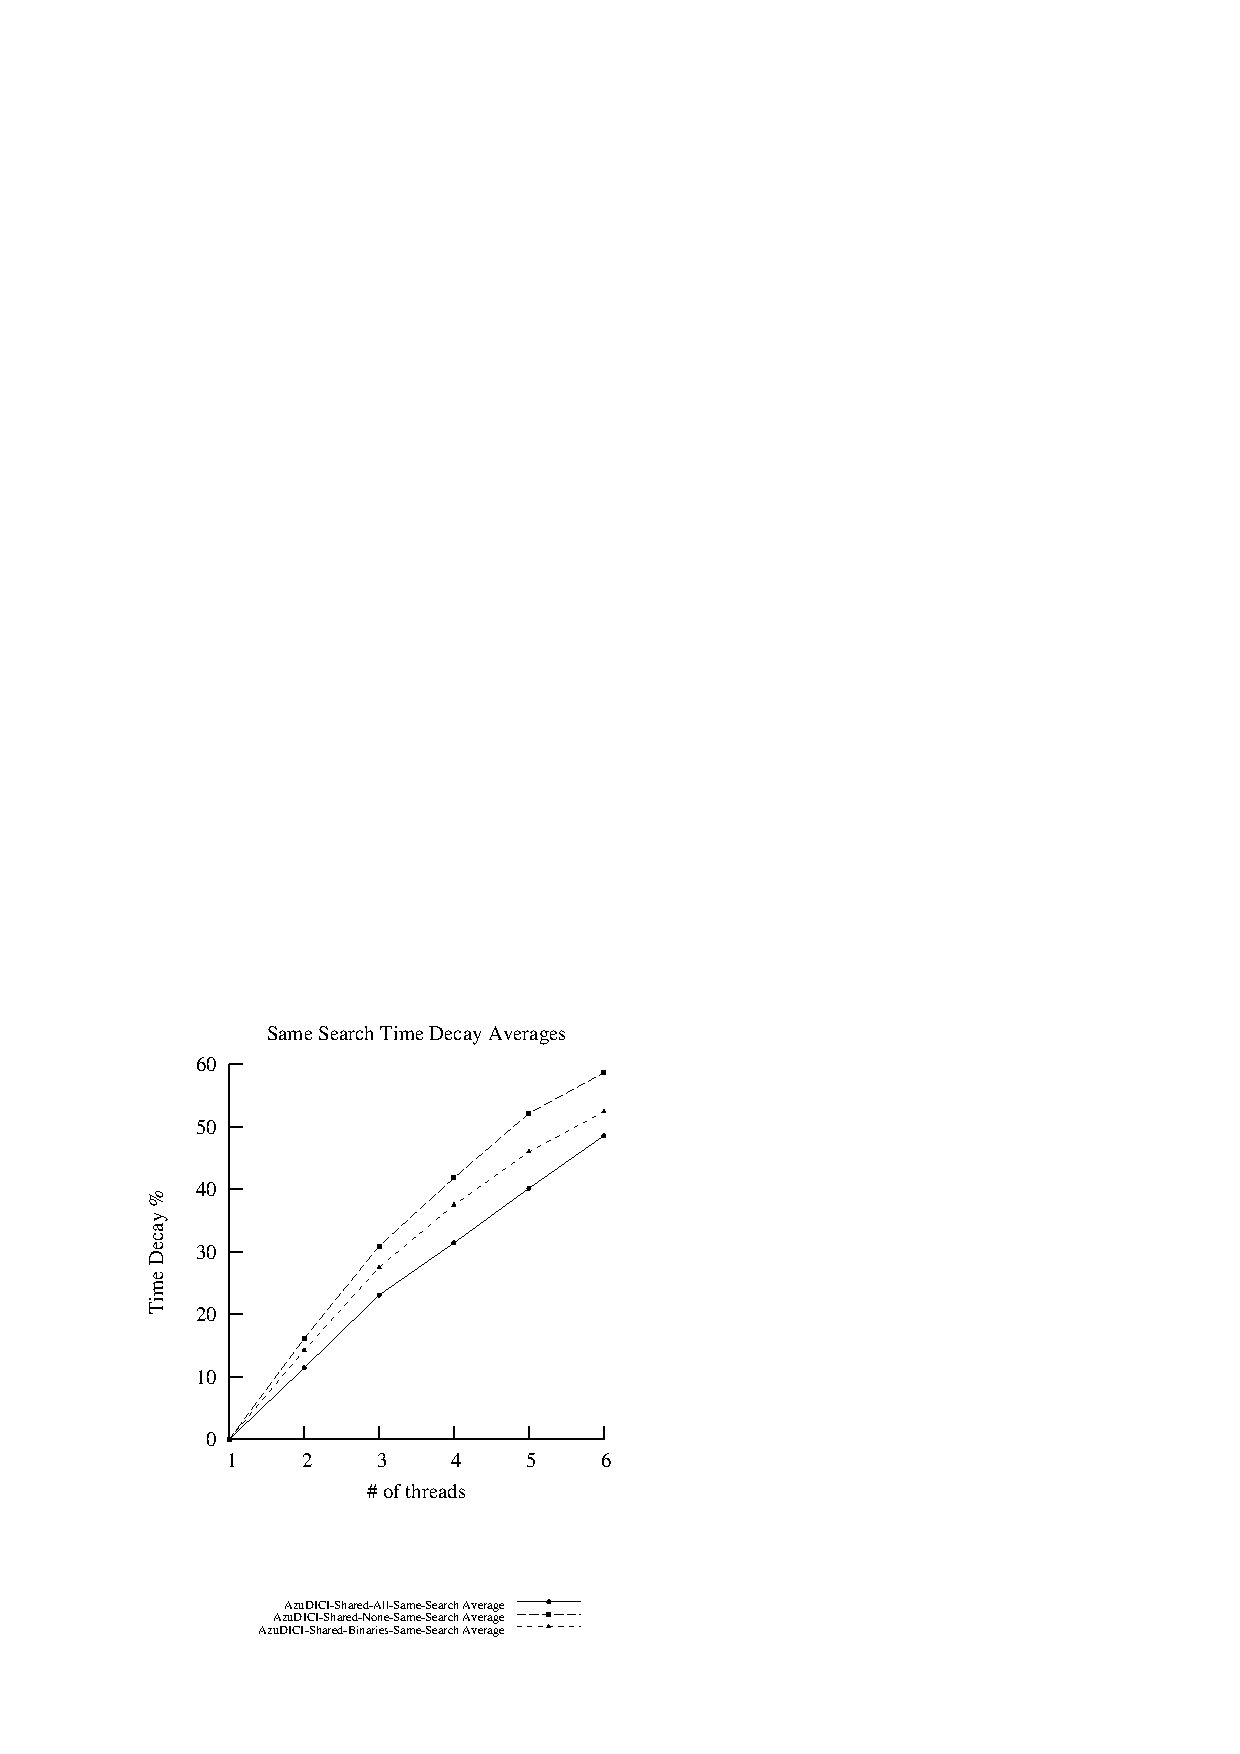
\includegraphics[scale=1]{averageSStime}
  \caption{Average running time for AZUDici version and number of
    threads}
  \label{fig:ssruntimes}
\end{figure}

\begin{figure}[htp]
  \centering
  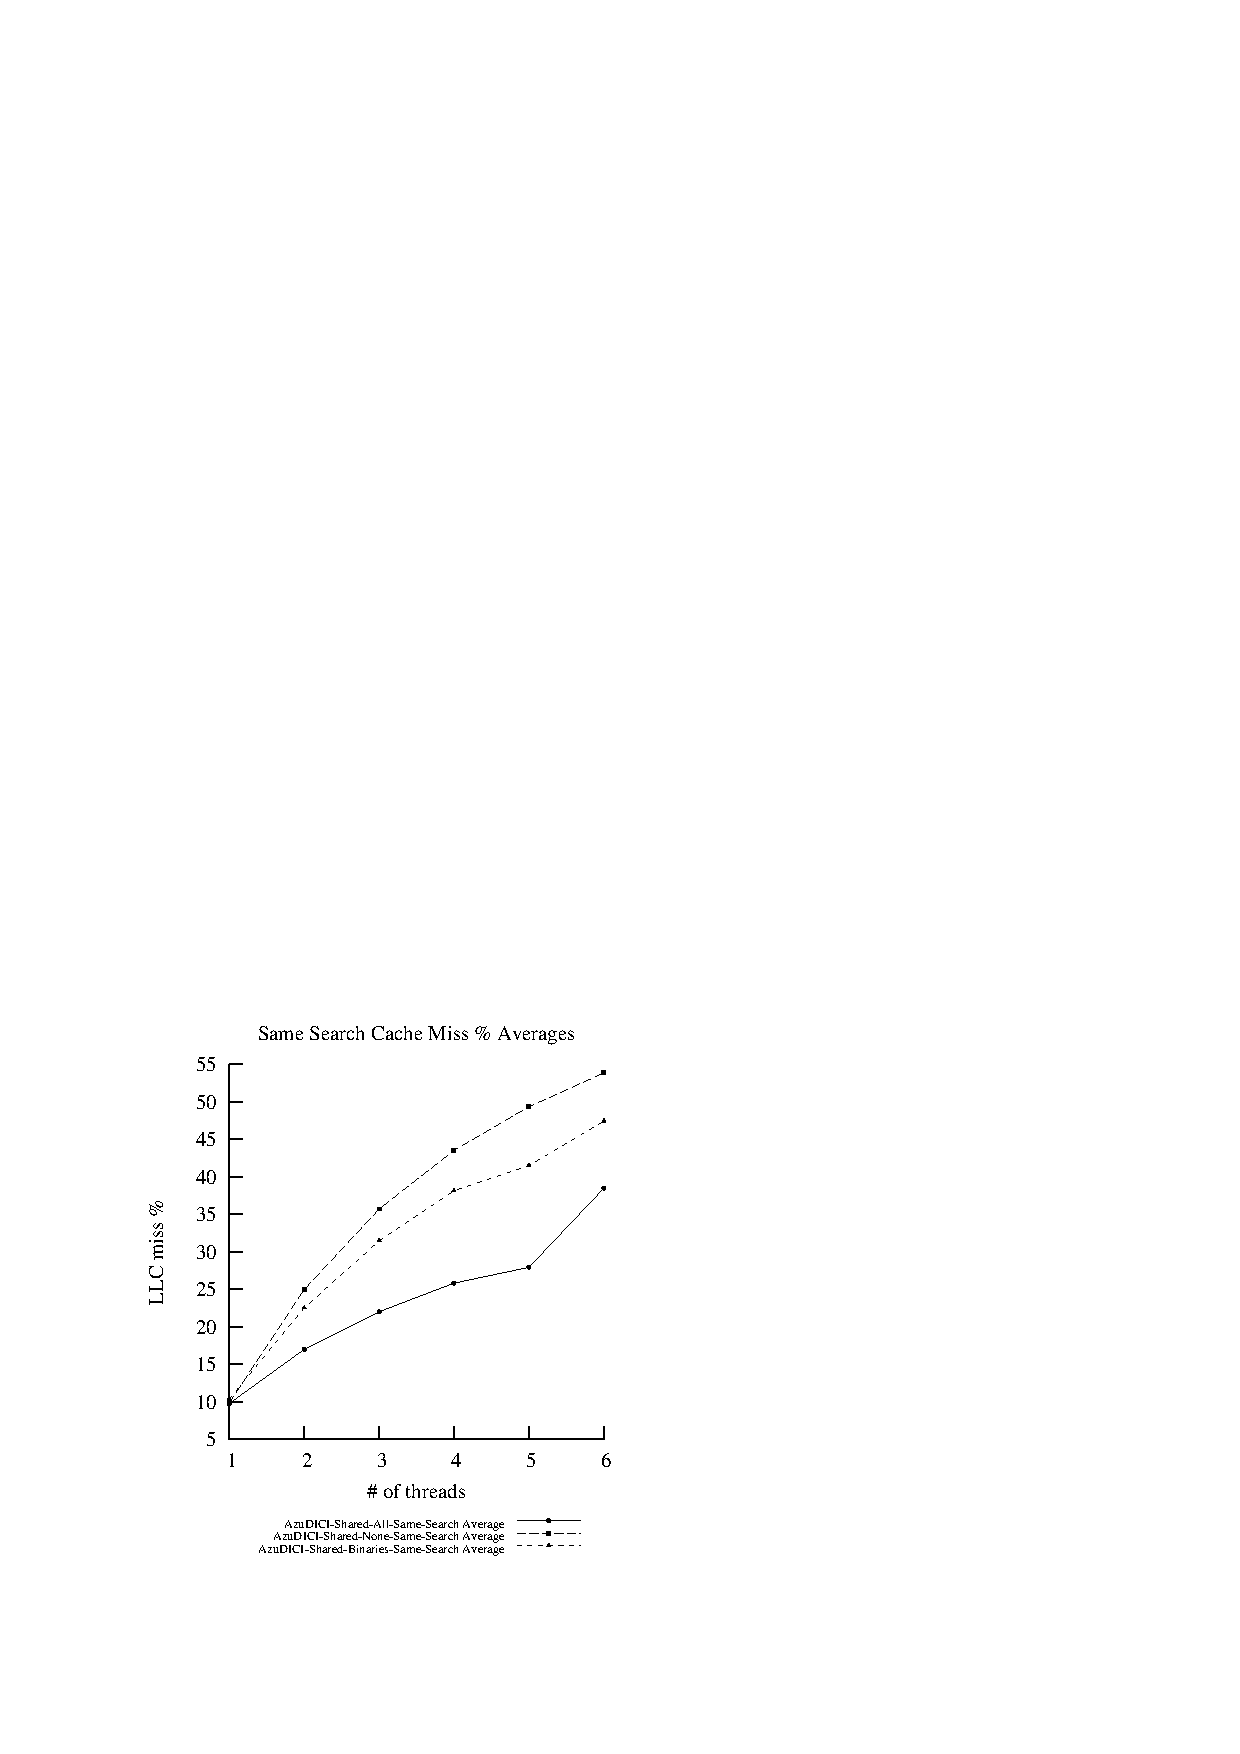
\includegraphics[scale=1]{averageSS}
  \caption{Average cache misses for AZUDici version and number of
    threads}
  \label{fig:sscachemisses}
\end{figure}

On aggregate, comparing the performance of AzuDICI as shown in Figure
\ref{fig:ssruntimes} and \ref{fig:sscachemisses}, it is evident that
the solver performs best in the shared-all condition, followed by the
shared-binary and finally by the shared-none condition in both running
time and cache misses. Thus, our implementation shows that physically
sharing the clause database is beneficial to avoid cache contention in
the rather artificial case of same search.

\subsection{Different search experiments}
\label{sec:diffsearch}

Our previous experiment validates our implementation of the
solver. Nonetheless, the results are not generalizable to a
full-featured SAT solver. It may be the case that while threads are
carrying out the same search, it is more likely that they will access
the same data. Whereas different search threads are clearly not
necessarily accessing the same data at the same time.

To find out how a real portfolio-approach SAT solver implementing
different levels of physical clause sharing behave, we ran AzuDICI in
the same three different versions as before (sharing-all, share-none
and share-bin) on the eight problems introduced in Section
\ref{sec:modifiedpling} using one to six threads and a 5-minute
timeout (we therefore did not include a running time table and
graph). The timeout characteristics was due to the fact that different
searches among threads may result in different (potentially better)
strategies, affecting execution time and rendering search behavior
effectively incomparable. Each run was repeated five times to clean up
potential system noise. XXXKeiraXXX


  \bgroup
  \def\arraystretch{1.5}

	\begin{table}[htbp]
	 \footnotesize
    \centering
		\begin{tabular}[h]{rcccccc} \hline
      Dataset  &  T1   & T2    & T3    &  T4   &  T5   &  T6 \\ \hline
	  \multirow{3}{*}{step17}		 &  3.0(5.2)		 &  7.5(0.6)		 &  14.0(0.3)		 &  21.5(0.3)		 &  27.3(0.2)		 &  34.1(0.1)		 \\
      &  2.9(1.4)		 &  6.4(3.8)		 &  13.9(2.7)		 &  17.8(3.0)		 &  25.5(1.1)		 &  31.2(1.5)		 \\
      &  2.8(0.9)		 &  5.8(2.0)		 &  12.3(1.8)		 &  16.5(1.4)		 &  22.6(0.2)		 &  29.0(1.3)		 \\ \hline
	  \multirow{3}{*}{E02F22}		 &  31.8(0.4)		 &  44.0(0.1)		 &  48.5(0.0)		 &  53.8(0.0)		 &  58.0(0.0)		 &  62.6(0.1)		 \\
      &  26.8(0.2)		 &  40.9(5.1)		 &  47.5(3.4)		 &  54.7(1.5)		 &  58.9(2.3)		 &  62.3(1.9)		 \\
      &  30.9(0.1)		 &  40.2(2.7)		 &  48.7(3.1)		 &  52.8(1.9)		 &  57.3(1.6)		 &  60.4(2.2)		 \\ \hline
	  \multirow{3}{*}{y-3.035}		 &  0.2(3.5)		 &  0.5(1.4)		 &  0.5(0.9)		 &  0.7(2.1)		 &  0.8(2.9)		 &  1.0(7.0)		 \\
      &  0.2(8.5)		 &  0.7(4.3)		 &  0.9(1.4)		 &  1.0(3.9)		 &  1.1(3.4)		 &  1.4(2.2)		 \\
      &  0.3(1.1)		 &  0.3(1.4)		 &  0.6(4.2)		 &  0.9(4.4)		 &  1.1(4.0)		 &  1.4(7.7)		 \\ \hline
	  \multirow{3}{*}{k45}			 &  22.0(0.4)		 &  33.6(0.1)		 &  44.2(0.1)		 &  50.6(0.1)		 &  54.9(0.0)		 &  59.5(0.0)		 \\
      &  25.3(0.6)		 &  34.5(0.4)		 &  42.1(0.5)		 &  48.3(0.2)		 &  53.3(0.1)		 &  56.8(0.3)		 \\
      &  25.1(0.1)		 &  34.1(0.6)		 &  41.8(0.3)		 &  48.3(0.3)		 &  52.6(0.2)		 &  56.0(0.3)		 \\ \hline
	  \multirow{3}{*}{k50}			 &  12.8(0.3)		 &  27.0(0.0)		 &  35.9(0.1)		 &  44.8(0.0)		 &  49.3(0.1)		 &  54.0(0.0)		 \\
      &  14.0(0.6)		 &  26.0(0.9)		 &  35.8(0.7)		 &  40.9(1.3)		 &  46.7(0.2)		 &  49.8(0.5)		 \\
      &  15.0(0.3)		 &  26.8(1.3)		 &  36.2(0.3)		 &  41.9(0.1)		 &  46.6(0.4)		 &  50.6(0.3)		 \\ \hline
	  \multirow{3}{*}{md5\_48\_3}		 &  12.1(0.5)		 &  23.3(0.1)		 &  31.9(0.2)		 &  39.1(0.1)		 &  43.6(0.1)		 &  48.2(0.0)		 \\
      &  13.4(0.3)		 &  23.0(2.8)		 &  32.0(0.2)		 &  37.0(0.2)		 &  41.8(2.1)		 &  46.1(0.1)		 \\
      &  14.3(0.2)		 &  23.5(0.3)		 &  32.2(0.3)		 &  37.0(0.1)		 &  41.8(0.2)		 &  45.7(0.2)		 \\ \hline
	  \multirow{3}{*}{L150}			 &  23.1(0.8)		 &  39.0(0.2)		 &  50.2(0.0)		 &  58.2(0.1)		 &  62.1(0.0)		 &  66.0(0.0)		 \\
      &  35.8(0.1)		 &  43.0(1.2)		 &  52.8(1.5)		 &  57.9(0.3)		 &  62.3(0.8)		 &  66.8(0.3)		 \\
      &  34.5(0.3)		 &  36.6(2.8)		 &  50.4(1.3)		 &  56.0(0.5)		 &  61.2(0.7)		 &  63.6(0.5)		 \\ \hline
	  \multirow{3}{*}{aes-top30}		 &  11.5(0.7)		 &  20.4(0.2)		 &  29.3(0.1)		 &  36.8(0.1)		 &  42.3(0.1)		 &  47.7(0.1)		 \\
      &  12.2(0.2)		 &  17.8(0.8)		 &  26.2(0.5)		 &  32.1(0.2)		 &  37.8(0.4)		 &  42.9(0.3)		 \\
      &  13.2(0.2)		 &  18.3(0.2)		 &  26.3(0.2)		 &  31.7(0.4)		 &  37.4(0.3)		 &  42.1(0.2)		 \\ \hline
	  \multirow{3}{*}{traffic\_b}		 &  4.4(3.4)		 &  17.4(0.7)		 &  31.9(0.3)		 &  44.3(0.1)		 &  52.1(0.0)		 &  59.8(0.0)		 \\
      &  4.3(1.8)		 &  16.7(1.2)		 &  31.4(0.2)		 &  41.7(0.2)		 &  51.4(0.1)		 &  58.7(0.0)		 \\
      &  4.0(3.5)		 &  14.6(0.3)		 &  28.4(0.5)		 &  37.5(0.4)		 &  46.3(0.2)		 &  53.8(0.1)		 \\ \hline
	  \multirow{3}{*}{UCG-15-10p1}	 &  21.4(0.6)		 &  31.8(0.1)		 &  40.6(0.1)		 &  43.6(0.1)		 &  46.9(0.1)		 &  49.8(0.1)		 \\
      &  20.7(0.7)		 &  31.7(3.0)		 &  40.9(2.4)		 &  46.2(2.0)		 &  53.5(0.8)		 &  55.5(0.6)		 \\
      &  22.6(0.6)		 &  34.8(1.8)		 &  42.8(2.8)		 &  49.6(2.1)		 &  51.6(1.7)		 &  55.2(0.5)		 \\ \hline    \end{tabular}
    \normalsize
    \caption{LLC misses (\%) for AzuDICI version and number of threads (T). The first row of each dataset corresponds to Shared-None version, second row to Shared-Bin and third row to Shared-All  . Numbers in parenthesis are standard deviations in \%.}
    \label{tab:dstable}
  \end{table}
  
\begin{figure}[htp]
  \centering
  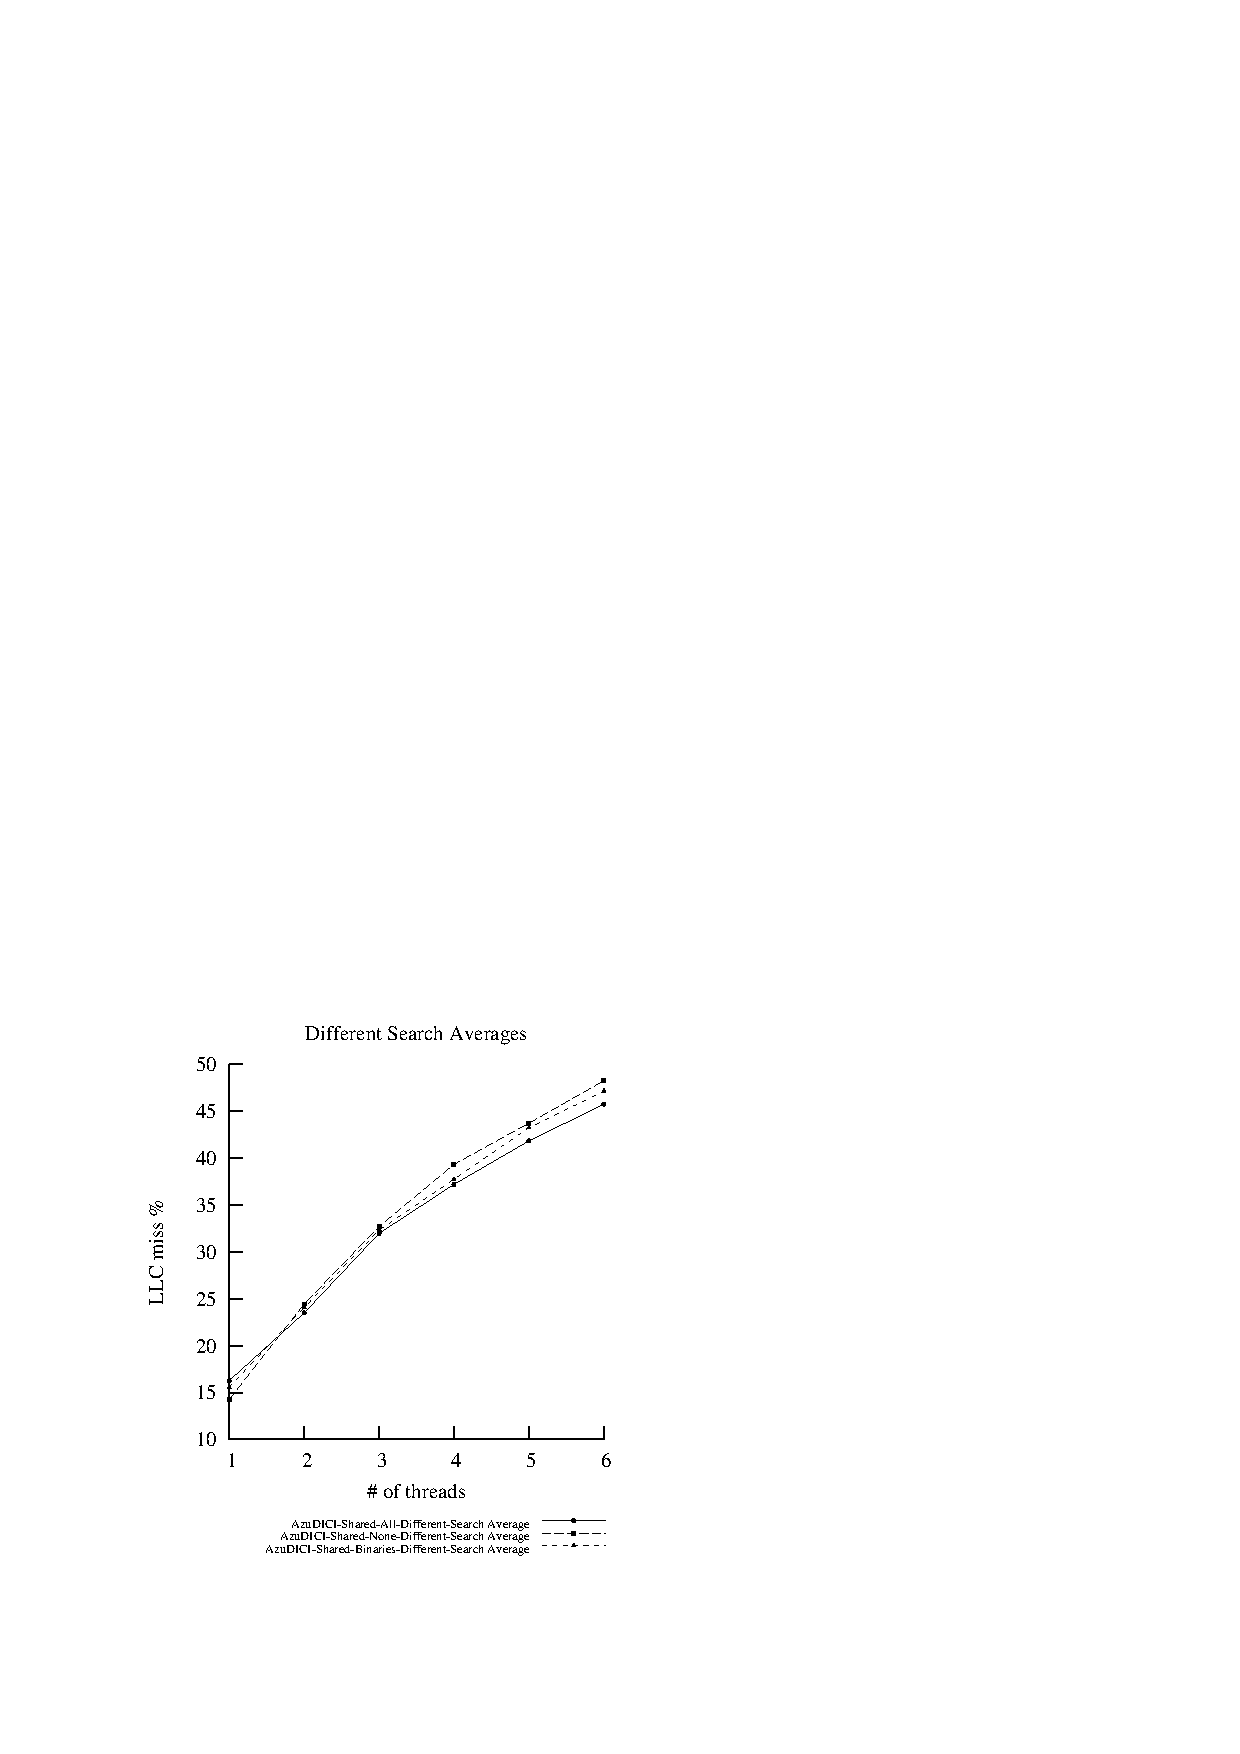
\includegraphics[scale=1]{averageDS}
  \caption{Average cache misses for AZUDici version and number of
    threads}
  \label{fig:dscachemisses}
\end{figure}

From these data, we may conclude that physically sharing the whole
clause database does not improve the cache performance of the
portfolio-approach-based SAT solvers

% Shared-all performs well wrt to cache misses, but that is not
% necessarily true for time. In general, the number of cache loads is
% larger when we are sharing the clause DB. Still, we think this is an
% implementation issue. That is, even if we may be saving on cache
% misses while sharing data, the more complex nature of the
% implementation can negatively influence overall time.

%%% Local Variables: 
%%% mode: latex
%%% TeX-master: "sat"
%%% End: 
